% The entire content of this work (including the source code
% for TeX files and the generated PDF documents) by 
% Hongxiang Chen (nicknamed we.taper, or just Taper) is
% licensed under a 
% Creative Commons Attribution-NonCommercial-ShareAlike 4.0 
% International License (Link to the complete license text:
% http://creativecommons.org/licenses/by-nc-sa/4.0/).
\documentclass{article}

\usepackage{float}  % For H in figures
\usepackage{amsmath} % For math
\usepackage{amssymb}
\usepackage{bbm} % for numbers within mathbb
\usepackage{mathrsfs} % For \mathscr{ABC}
% Followings are for the special character: differential "d".
\newcommand*\diff{\mathop{}\!\mathrm{d}}
\newcommand*\Diff[1]{\mathop{}\!\mathrm{d^#1}}
\numberwithin{equation}{subsection} % have the enumeration go to the subsection level.
                                    % See:https://en.wikibooks.org/wiki/LaTeX/Advanced_Mathematics
\usepackage{graphicx}   % need for figures
\usepackage{cite} % need for bibligraphy.
\usepackage[unicode]{hyperref}  % make every cite a link
\usepackage{CJKutf8} % For Chinese characters
\usepackage{fancyref} % For easy adding figure,equation etc in reference. Use \fref or \Fref instead of \ref

% Following is for theorems etc environments
% http://tex.stackexchange.com/questions/45817/theorem-definition-lemma-problem-numbering && https://en.wikibooks.org/wiki/LaTeX/Theorems
\usepackage{amsthm}
\newtheorem{defi}{Definition}[section]
\newtheorem{thm}{Theorem}[section]
\newtheorem{lemma}{Lemma}[section]
\newtheorem{remark}{Remark}[section]
\newtheorem{prop}{Proposition}[section]
\newtheorem{coro}{Corollary}[section]
\newtheorem{fact}{Fact}[section]
\theoremstyle{definition}
\newtheorem{ex}{Example}[section]
\newtheorem{argument}{Argument}[section]

% A list of nomenclatures.
\usepackage{nomencl}
\makenomenclature

% For drawing diagrams with arrows
\usepackage[all]{xy}

% For highlighting
\usepackage{color,soul}

% Resolving pdf version warning
\pdfoptionpdfminorversion=7

% My own physics package
% The following line load the package xparse with additional option to
% prevent the annoying warnings, which are caused by the package
% "physics" loaded in package "physics-taper".
\usepackage[log-declarations=false]{xparse}
\usepackage{physics-taper}

\title{General Physics Formula}
\date{\today}
\author{Taper}


\begin{document}


\maketitle
\abstract{
This is a collection of important formulae in Fundamentals of Physics
Extended Version by Halliday and Resnick, and some other formulae from
other sources. Although this was initially intended to be preparation
for GRE physics exam, I found such a review quite useful and will
continue to update this document whenever I found something useful.
}
\tableofcontents

\section{General}
\label{sec:Table}

\begin{table}[H]
    \centering
    \caption{Metric Prefix}
    \begin{tabular}{c c c}
        tera  & T     & $10^{12}$ \\
        giga  & G     & $10^{9}$ \\
        mega  & M     & $10^{6}$ \\
        kilo  & k     & $10^{3}$ \\
        centi & c     & $10^{-2}$ \\
        milli & m     & $10^{-3}$ \\
        micro & $\mu$ & $10^{-6}$ \\
        nano  & n     & $10^{-9}$ \\
        pico  & p     & $10^{-12}$ \\
    \end{tabular}
\end{table}

\paragraph{Rotation matrix}
Active rotation in the bbb counter-clockwise $\theta$:
\begin{equation}
    \left(
    \begin{array}{cc}
        \cos{\theta} & -\sin{\theta} \\
        \sin{\theta} & \cos{\theta} \\
    \end{array}
    \right)
\end{equation}

\subsection{Fourier Transformation}
\label{sec:Fourier-Transformation}
From
\href{http://mathworld.wolfram.com/DeltaFunction.html}{Delta Function
- Wolfram Mathworld}.
\begin{align}
    \delta(x) &= \mathcal{F}_k[1](x) = \int_{-\infty}^{\infty}
        e^{-2\pi i kx} \dd k \\
    1 &= \mathcal{F}^{-1}[\delta(x)](k) = \int_{-\infty}^{\infty}
        \delta(x) e^{2\pi ikx}\dd x= 1
\end{align}



\section{Classical mechanics}
\label{sec:Classical-mechanics}

\begin{align}
L &= T- V\\
\frac{\diff}{\diff t} \left(\frac{\partial L}{\partial \dot{q}}\right)
    &= \frac{\partial L}{\partial q} \\
\dot{q} &= \frac{\partial H}{\partial p} \\
\dot{p} &= -\frac{\partial H}{\partial q}
\end{align}

\paragraph{Constant Accleration}
These five equations in Table 2-1 describe the motion of a particle with constant acceleration:
\begin{align}
    v           &= v_0 + at \\
    x-x_0       &= v_0 t + \frac{1}{2} at^2\\
    x-x_0       &= vt - \frac{1}{2} at^2\\
    v^2 - v_0^2 &= 2a(x-x_0)\\
    x-x_0       &= \frac{1}{2} (v_0+v) t
\end{align}

\paragraph{Projectile Motion} Projectile motion is the motion of a
particle that is launched with an initial velocity $\vec v_0$. During
its flight, the particle’s horizontal acceleration is zero and its
vertical acceleration is the free-fall acceleration $-g$. (Upward is
taken to be a positive direction.) If $\vec v_0$ is expressed as a
magnitude (the speed $v_0$) and an angle $\theta_0$ (measured from the
horizontal), the particle’s equations of motion along the horizontal x
axis and vertical y axis are
\begin{align}
    x-x_0 &= (v_0 \cos(\theta_0) ) t \\
    y-y_0 &= (v_0 \sin(\theta_0) ) t - \frac{1}{2} gt^2 \\
    v_y   &= v_0 \sin{\theta_0} - gt \\
    v_y^2 &= (v_0 \sin{\theta_0})^2 - 2g (y-y_0)
\end{align}
The \textbf{trajectory} (path) of a particle in projectile motion is
parabolic and is given by
\begin{align}
    y &= (\tan{\theta_0}) x - \frac{gx^2}{2(v_0 \cos{\theta_0})^2} 
\end{align}

\paragraph{Uniform Circular Motion} If a particle travels along a circle
or circular arc of radius $r$ at constant speed $v$, it is said to be in
\textit{uniform circular motion} and has an acceleration of constant
magnitude
\begin{align}
    a = \frac{v^2}{r}
\end{align}
The direction of is toward the center of the circle or circular arc,
and is said to be centripetal. The time for the particle to complete
a circle is
\begin{align}
    T=\frac{2\pi r}{v}
\end{align}
$T$ is called the period of revolution, or simply the period, of the
motion.

This acceleration is due to a net centripetal force on the particle,
with magnitude given by
\begin{align}
    F = \frac{mv^2}{R}
\end{align}
where $m$ is the particle’s mass. The vector quantities $\vec a$ and
$\vec F$ are directed toward the center of curvature of the particle’s
path

\paragraph{First, Second Speed}

\textbf{Circular}: $v = \sqrt{gR}$.

\textbf{Escape Speed} $\frac{1}{2}mv^2 = \frac{GMm}{R}$, so
$v=\sqrt{2GM/R}$.
\begin{defi}[Normal force]
\nomenclature{Normal force}{\nomrefpage.}
A \textbf{normal force} is the force on a body from a surface against
which the body presses.The normal force is always perpendicular to the
surface.
\end{defi}

\paragraph{Drag Force} When there is relative motion between air (or
some other fluid) and a body, the body experiences a drag force $\vec
D$
that opposes the relative motion and points in the direction in
which the fluid flows relative to the body. The magnitude of $\vec D$is
related to the relative speed $v$ by an experimentally determined
drag coefficient $C$ according to
\begin{align}
    D=\frac{1}{2} C\rho A v^2
\end{align}
where $\rho$ is the fluid density (mass per unit volume) and $A$ is
the effective cross-sectional area of the body (the area of a cross
section taken perpendicular to the relative velocity $\vec v$)

Power The power due to a force is the rate at which that force
does work on an object. For a force $\vec F$ at an angle $\phi$ to the
direction of travel of the instantaneous velocity $\vec v$, the
instantaneous power is
\begin{align}
    P = Fv \cos{\phi} = \vec{F} \cdot \vec{v}
\end{align}

\paragraph{Collision and Impulse} Applying Newton’s second law in
momentum form to a particle-like body involved in a collision
leads to the impulse–linear momentum theorem:
\begin{align}
    \vec{p}_f - \vec{p}_i = \int_{t_i}^{t_f} \vec{F} \diff t
\end{align}
where the LHS is the change in the body’s linear
momentum, and RHS is defined as the impulse $\vec{J}$ due to the force
exerted on the body by the other body in the collision.

\paragraph{Elastic Collisions in One Dimension} An elastic collision
is a special type of collision in which the kinetic energy of a system
of colliding bodies is conserved. If the system is closed and
isolated, its linear momentum is also conserved. For a one-dimensional
collision in which body $2$ is a target and body $1$ is an incoming
projectile, conservation of kinetic energy and linear momentum yield
the following expressions for the velocities immediately after the
collision:
\begin{align}
    v_{1f} &= \frac{m_1-m_2}{m_1+m_2} v_{1i} \\
    v_{2f} &= \frac{2m_1}{m_1+m_2} v_{1i}
\end{align}

Variable-Mass Systems In the absence of external forces a rocket
accelerates at an instantaneous rate given by
\begin{align}
    R v_{\text{rel}} = Ma \text{(first rocket equation)}
\end{align}
in which $M$ is the rocket’s instantaneous mass (including
unexpended fuel), $R$ is the fuel consumption rate, and $v_{\text{rel}}$ is the fuel’s
exhaust speed relative to the rocket. The term $R v_{\text{rel}}$ is the thrust of
the rocket engine. For a rocket with constant R and $v_{\text{rel}}$, whose speed
changes from $v_i$ to $v_f$ when its mass changes from $M_i$ to $M_f$,
\begin{align}
    v_f - v_i = v_{\text{rel}} \ln\frac{M_i}{M_f} \text{(second rocket
    equation)}
\end{align}
($R\equiv |\frac{\diff M}{\diff t}|$)

\paragraph{The Kinematic Equations for Constant Angular Acceleration}
Constant angular acceleration ($\alpha =$a constant) is an important
special case of rotational motion. The appropriate kinematic
equations, given in Table 10-1, are
\begin{align}
    \sigma &= \sigma_0 + \alpha t \\
    \theta - \theta_0 &= \omega_0 t + \frac{1}{2} \alpha t^2 \\
    \theta - \theta_0 &= \omega t - \frac{1}{2} \alpha t^2 \\
    \omega^2 - \omega_0^2 &= 2\alpha (\theta - \theta_0) \\
    \theta - \theta_0 &= \frac{1}{2}(\omega_0 + \omega) t
\end{align}

\paragraph{Linear and Angular Variables Related} A point in a rigid
rotating body, at a perpendicular distance $r$ from the rotation axis,
moves in a circle with radius $r$. 

The linear acceleration $\vec{a}$ of the point \hl{has both tangential and
radial components}.The tangential component is
\begin{align}
    a_t = \alpha r
\end{align}
where $\alpha$ is the magnitude of the angular acceleration (in radians
per second-squared) of the body.The radial component of $\vec{a}$ is
\begin{align}
    a_r = \frac{v^2}{r} = \omega^2 r
\end{align}
If the point moves in uniform circular motion, the period $T$ of
the motion for the point and the body is
\begin{align}
    T = \frac{2\pi r}{v} = \frac{2\pi}{\omega}
\end{align}
\paragraph{Rotational Kinetic Energy and Rotational Inertia} The
kinetic energy $K$ of a rigid body rotating about a fixed axis is
given by
\begin{align}
    K=\frac{1}{2} I\omega^2
\end{align}
in which $I$ is the rotational inertia of the body, defined as
\begin{align}
    I \equiv \int r^2 \diff m
\end{align}
\paragraph{The Parallel-Axis Theorem} 265
\begin{align}
    I = I_{\text{com}} + M h^2
\end{align}
\begin{figure}[H]
    \centering
    \includegraphics[width=0.8\linewidth]{pics/{some-rotational-inertias}.png}
    \caption{Some Rotational Inertias (p. 255 of\cite{book}) }
    \label{fig:some-rotational-inertias}
\end{figure}
\paragraph{Work and Rotational Kinetic Energy} 265
\begin{align}
    W = \int_{\theta_i}^{\theta_f} \tau \diff \theta \\
    P = \frac{\diff W}{\diff t} = \tau \omega
\end{align}

\paragraph{Rolling Bodies}
[295]
\begin{align}
    v_\text{com} &= \omega R\\
    K  &= \frac{1}{2}I_\text{com}\omega^2 + \frac{1}{2}Mv_\text{com}^2
    \\
    a_\text{com} = \alpha R
\end{align}
\paragraph{Precession of a Gyroscope}
\begin{align}
    \Omega = \frac{Mgr}{I\omega}
\end{align}

\paragraph{Elastic Moduli} [319]
\begin{center}
    stress $=$ modulus $\times$ strain
\end{center}

Young's modulus:
\begin{align}
    \frac{F}{A} = E \frac{\Delta L}{L}
\end{align}

Shear's modulus:
\begin{align}
    \frac{F}{A} = G \frac{\Delta x}{L}
\end{align}

Hydraulic bulk modulus:
\begin{align}
    p = B \frac{\Delta V}{V}
\end{align}

\paragraph{Gravitational Potential Energy} [349]
\begin{align}
    U = -\frac{GMm}{r}
\end{align}

\textbf{Escape speed}
\begin{align}
    v = \sqrt{ \frac{2GM}{R} }
\end{align}

\textbf{Kepler's Laws}
\begin{enumerate}
    \item The law of orbits. All planets move in elliptical orbits
        with the Sun at one focus.
    \item The law of areas. A line joining any planet to the Sun
        sweeps out equal areas in equal time intervals. (This
        statement is equivalent to conservation of angular momentum.)
    \item The law of periods. The square of the period $T$ of any
        planet is proportional to the cube of the semimajor axis a of
        its orbit. For circular orbits with radius $r$,
    \begin{align}
        T^2 = \left(\frac{4\pi^2}{GM}\right) r^3
    \end{align}
        where $M$ is the mass of the attracting body—the Sun in the
        case of the solar system. For elliptical planetary orbits, the
        semimajor axis $a$ is substituted for $r$.
\end{enumerate}

\textbf{Energy in Planetary Motion}
\begin{align}
    U &= -\frac{GMm}{r} \\
    K &= \frac{GMm}{2r} \\
    E &= -\frac{GMm}{2r} \,\text{ or} \\
    E &= -\frac{GMm}{2a} 
\end{align}

\section{Fluid}
\label{sec:Fluid}

\paragraph{Flow of Ideal Fluids}[377]
\begin{defi}[Apparent weight]
\nomenclature{Apparent weight}{\nomrefpage.}
    Omited
\end{defi}

\textbf{Equation of continuity}
\begin{align}
    R_v \equiv Av = \text{ a constant}
\end{align}
\textbf{Bernoulli's Equation}
\begin{align}
    p + \frac{1}{2}\rho v^2 + \rho gh = \text{ a constant}
\end{align}

\section{Wave}
\label{sec:Wave}

\paragraph{Oscillation} (\textbf{pp.403 of \cite{book}})
\begin{align}
    \omega &= \frac{2\pi}{T} = 2\pi f
\end{align}
\textbf{Linear Oscillator}
\begin{align}
    & \omega = \sqrt{\frac{k}{m}} \\
    & T = 2\pi \sqrt{\frac{m}{k}} 
\end{align}
\textbf{Pendulums}
\begin{align}
    & T = 2\pi \sqrt{I/\kappa} \\
    & T = 2\pi \sqrt{L/g} \\
    & T = 2\pi \sqrt{I/mgh}
\end{align}
\textbf{Damped Harmonic Motion}
\begin{align}
    & x(t) = x_m e^{-bt/2m} \cos\left( \omega' t+\phi\right) \\
    & \omega' = \sqrt{ \frac{k}{m} - \frac{b^2}{4m^2} } \\
    & E(t)\approx \frac{1}{2} kx_m^2 e^{-bt/m}
\end{align}


\paragraph{Waves} (\textbf{pp.436 ch16 of \cite{book}})
\begin{align}
    & y(x,t) = y_m \sin(kx-\omega t) \\
    & k = \frac{2\pi}{\lambda} \\
    & f = \frac{\omega}{2\pi} = \frac{1}{T} \\
    & v = \frac{\omega}{k} = \frac{\lambda}{T} = \lambda f
\end{align}

\begin{figure}[H]
    \centering
    \includegraphics[width=0.8\linewidth]{pics/{wave-and-reflection}.PNG}
    \caption{wave and Reflection}
\end{figure}
$(a)$ A pulse incident from the right is reflected at the left end of
the string, which is tied to a wall. Note that the reflected pulse is
inverted from the incident pulse. $(b)$ Here the left end of the string
is tied to a ring that can slide without friction up and down the rod.
Now the pulse is not inverted by the reflection

\textbf{String}
\begin{align}
    & v = \sqrt{\frac{\tau}{\mu}} \\
    & P_\text{avg} = \frac{1}{2}\mu v \omega^2 y_m^2
\end{align}
\textbf{Resonance}
\begin{align}
    n \lambda = 2L
\end{align}
\paragraph{Sound (Longitudinal) Wave} (\textbf{pp.466 ch17 of
\cite{book}})
\begin{align}
    & v = \sqrt{\frac{B}{\rho}} \\
    & s = s_m \cos(kx-\omega t) \\
    & \Delta p = \Delta p_m sin(kx-\omega r) \\
    & \Delta p_m = (v\rho \omega) s_m
\end{align}
\textbf{Sound Intensity}
\begin{align}
    & I = \frac{P}{A} \\
    & I = \frac{1}{2}\rho v \omega^2 s_m^2 \\
    & I = \frac{P_s}{4\pi r^2} \\
\end{align}
\textbf{Standing Wave Patterns in Pipes}
\begin{align}
    & f = \frac{v}{\lambda} = \frac{nv}{2L}\text{, $n=1,2,3,\cdots$} \\
    & f = \frac{v}{\lambda} = \frac{nv}{4L}\text{, $n=1,3,5,\cdots$}
\end{align}
\begin{figure}[H]
    \centering
    \includegraphics[width=0.8\linewidth]{pics/{ch17.sound_wave}.png}
\end{figure}
\textbf{Beat}
\begin{align}
    f_\text{beat} = f_1 - f_2
\end{align}
\textbf{The Doppler Effect}
\begin{align}
    f' = f \frac{ v \pm v_D}{ v\pm v_s}
\end{align}
The signs are chosen such that $f'$ tends to be \textit{greater} for
motion toward and \textit{less} for motion away.
\textbf{Shock wave}
\begin{align}
    \sin{\theta} = \frac{v}{v_s}\text{ , $v_s\geq v$}
\end{align}

\section{Thermal Physics}
\label{sec:Thermal-Physics}

\paragraph{Conduction} (\textbf{pp.498 ch18 of \cite{book}})
\textbf{Thermal expansion}
\begin{align}
    & \Delta L = L \alpha \Delta T \\
    & \Delta V = V \beta \Delta T \\
    & \beta = 3 \alpha \\
    & Q = C \Delta T = cm \Delta T
\end{align}
\begin{defi}[Convection]
\nomenclature{Convection}{\nomrefpage.}
    Convection occurs when temperature differences cause an energy
    transfer by motion within a fluid
\end{defi}
\textbf{Radiation}
\begin{align}
    & P_\text{rad} = \sigma \varepsilon AT^4 \\
    & P_\text{abs} = \sigma \varepsilon AT_\text{evn}^4
\end{align}

\textbf{Black Body Radiation}
Plank's law:
\begin{equation}
    I(\mu,T) = \frac{2h\mu^3}{c^2} \frac{1}{e^{\frac{h\mu}{kT}-1}}
\end{equation}
Wien's displacement law:

Wien's displacement law shows how the spectrum of black-body radiation
at any temperature is related to the spectrum at any other
temperature. If we know the shape of the spectrum at one temperature,
we can calculate the shape at any other temperature. Spectral
intensity can be expressed as a function of wavelength or of
frequency.

A consequence of Wien's displacement law is that the wavelength at
which the intensity per unit wavelength of the radiation produced by a
black body is at a maximum, $\lambda_\text{max}$, is a function only of the temperature:
\begin{equation}
    \lambda_\text{max}=\frac{b}{T}
\end{equation}
where the constant $b$, known as Wien's displacement constant.
\textbf{Conduction}
\begin{align}
    & P_\text{cond} \equiv \frac{Q}{t} = kA \frac{T_H-T_C}{L}  \\
    & P_\text{cond} = A \frac{T_H-T_C}{\sum(L_i/K_i)}
\end{align}
\begin{figure}[H]
    \centering
    \includegraphics[width=0.8\linewidth]{pics/{ch18.heat_cond}.png}
    \caption{pp.494 of \cite{book}}
\end{figure}
\begin{figure}[H]
    \centering
    \includegraphics[width=0.8\linewidth]{pics/{ch18.heat_cond_series}.png}
    \caption{pp.495 of \cite{book}}
\end{figure}

\paragraph{Thermal Process} (\textbf{pp.529 ch19 of \cite{book}})
Thermal process:
\begin{table}[H]
    \centering
    \begin{tabular}{|c|c|c|c|}
        \hline
        No. & Constant Quaility            & Process Type & Special Results  \\
        \hline
        1   & $p$                          & Isobaric     & $Q = nC_p\Delta T;W=p\Delta V$ \\
        2   & $T$                          & Isothermal   & $Q=W=nRT\ln(V_f/V_i); \Delta E_\text{int}=0$  \\
        3   & $pV^\gamma$, $TV^{\gamma-1}$ & Adiabatic    & $W=-\Delta E_\text{int}$ \\
        4   & $V$                          & Isochoric    & $Q=\Delta E_\text{int}=nC_V \Delta T;W=0$ \\
        \hline
    \end{tabular}
\end{table}
In particular, for Adiabatic process (let $K\equiv pV^\gamma$):
\begin{equation}
    W = \int_i^f \frac{K}{V^\gamma}\dd V =
    \frac{p_fV_f-p_iV_i}{1-\gamma}
\end{equation}
\begin{figure}[H]
    \centering
    \includegraphics[width=0.8\linewidth]{pics/{ch18.therm_pro}.png}
\end{figure}
Isothermal Process:
\begin{align}
    W = Nk T \ln\frac{V_f}{V_i}
\end{align}
\textbf{Temperature and Kinetic Energy}
\begin{align}
    & K_\text{avg} = \frac{3}{2}kT \text{, per molecule} \\
    & \lambda = \frac{1}{\sqrt{2} \pi d^2 N/V} 
\end{align}
\paragraph{Molar Specific Heats}
\begin{align}
    & C_V = \frac{3}{2} R \\
    & C_P = C_V + R \\
    & \Delta E_\text{int} = N C_V \Delta T \\
    & C_V = \frac{f}{2} k \\
    & \gamma \equiv \frac{C_P}{C_V}
\end{align}

Even more accurate formulae found in pp. 158 Kardar's book \cite{kardar}:
\begin{align}
    & C_V = \frac{6n-3-r}{2}k_B \\
    & C_p = C_V + k_B
\end{align}
\begin{figure}[H]
    \centering
    \includegraphics[width=0.8\linewidth]{pics/{kardar-C_v-formulae}.PNG}
    \caption{Examples of $n,r,$ and $\gamma$.}
\end{figure}
But these are \hl{\textbf{classical results}}, only valid at high
temperature! (See the refered page for details).

\paragraph{Entropy} (\textbf{pp.554 ch20 of \cite{book}})

\begin{align}
    & \diff S = \frac{\diff Q}{T} \\
    & \Delta S = nR \ln{\frac{V_f}{V_i}} + nC_V \ln{\frac{T_f}{T_i}}
    \\
    & \varepsilon = 1-\frac{T_L}{T_H}  \text{ (Carnot engine)} \\
    & K = \frac{T_L}{T_H-T_L} \text{ (Carnot refrigerator)}  \\
    & \ln{N!} \approx N\ln{N} - N
\end{align}

\section{Electrodynamics}
\label{sec:Electrodynamics}

\paragraph{Lorentz Force Law}
\begin{equation}
    \vb{F} = q\left(\vb{E} +\vb{v}\cross\vb{B}\right)
\end{equation}
\paragraph{Electric field} (\textbf{pp.596 ch22 of \cite{book}})
\begin{align}
    & E = \frac{1}{4\pi \varepsilon_0} \frac{q}{r^2} \\
    & E = \frac{1}{2\pi \varepsilon_0} \frac{p}{z^3} \\
    & U = - \vec{p}\cdot \vec{E} 
\end{align}

\paragraph{Gauss's Law} (\textbf{pp.620 ch23 of \cite{book}})

\begin{align}
    & E = \frac{\sigma}{\varepsilon_0}\text{ ,charged conductor} \\
    & E = \frac{\sigma}{2\varepsilon_0}\text{ ,infinite sheet} \\
    & E = \frac{\lambda}{2\pi\varepsilon_0 r} \\
    & E = 0 \text{ , inside charged shell} \\
    & E = \left(\frac{q}{4\pi\varepsilon_0 R^3}\right) r
\end{align}

\paragraph{Electric Potential} (\textbf{pp.646 ch24 of \cite{book}})

\begin{align}
    & V = \frac{1}{4\pi\varepsilon_0}\frac{q}{r} \\
    & V = \frac{1}{4\pi\varepsilon_0}\frac{p\cos\theta}{r^2} \\
    & U = \frac{1}{4\pi\varepsilon_0}\frac{q_1 q_2}{r}
\end{align}

\paragraph{Capacitor} (\textbf{pp.675 ch25 of \cite{book}})

\begin{align}
    & C \equiv \frac{q}{V} \\
    & C = \frac{\varepsilon_0 A}{d} \text{ (parallel-plate)} \\
    & C = 2\pi \varepsilon_0 \frac{L}{\ln{b/a}} 
            \text{ (cylindrical)}\\
    & C = 4\pi \varepsilon_0 \frac{ab}{b-a} \text{ (spherical)}\\
    & C = 4\pi \varepsilon_0 R \text{ (isolated spherical)} \\
    & C = \sum_j C_j \text{ (parallel)} \\
    & \frac{1}{C} = \sum_j \frac{1}{C_j} \text{ (series)}  \\
    & U = \frac{1}{2}\frac{q^2}{C} = \frac{1}{2}CV^2 \\
    & u = \frac{1}{2}\varepsilon_0 E^2
\end{align}

\paragraph{Current} (\textbf{pp.698 ch26 of \cite{book}})

\begin{align}
    & \vec{J} = ne \vec{v}_d \\
    & \rho \equiv \frac{1}{\sigma} = \frac{E}{J} \\
    & \vec{E} = \rho \vec{J} \\
    & R = \rho \frac{L}{A} \\
    & \rho - \rho_0 = \rho_0 \alpha (T-T_0) \\
    & \rho = \frac{m}{e^2 n\tau }
\end{align}

\paragraph{Electro motive force} (\textbf{pp.724 ch27 of \cite{book}})

\begin{align}
    & \mathcal{E} = \frac{\diff W}{\diff q}
\end{align}
Cutting Magnetic field lines:
\begin{equation}
    \mathcal{E} = BLv 
\end{equation}
Cutting Magnetic field lines in circular motion:
\begin{equation}
    \mathcal{E} = B(\frac{1}{2}\omega R) R = \frac{1}{2}B\omega R^2
\end{equation}
For electric generator:
\begin{equation}
    E_\text{max} = nBA_\text{rea}\omega
\end{equation}
\textbf{Circuit Rule}
\begin{itemize}
    \item \textbf{Loop Rule}. The algebraic sum of the changes in
        potential encountered in a complete traversal of any loop of a
        circuit must be zero.
    \item \textbf{Junction Rule}. The sum of the currents entering any
        junction must be equal to the sum of the currents leaving that
        junction
\end{itemize}

\begin{align}
    & R = \sum_j R_j \text{ , series} \\
    & \frac{1}{R} = \sum_j \frac{1}{R_j} \text{ , parallel}
\end{align}

\paragraph{Magnetic Field} (\textbf{pp.755 ch28 of \cite{book}})

\begin{align}
    & qvB = \frac{mv^2}{r} \\
    & T = \frac{2\pi r}{ rqB / m} = \frac{2\pi m}{qB} \\
    & \vec\tau = \vec{\mu} \times \vec{B} \\
    & U(\theta) = -\vec\mu \cdot \vec B
\end{align}

\paragraph{Magnetic $\to$ Electricity} (\textbf{pp.781 ch29 of
\cite{book}})

\begin{align}
    & \diff \vec{B} = \frac{\mu_0}{4\pi}
        \frac{i\diff \vec{s}\times\hat{r}}{r^2} \\
    & B = \frac{\mu_0 i}{2\pi R} \\
    & B = \frac{\mu_0 i \phi}{4\pi R} \\
    & B = \mu_0 i N/L \\
    & B = \frac{\mu_i i N}{2\pi}\frac{1}{r} \\
    & \vec{B}(z) = \frac{\mu_0}{2\pi}\frac{\vec{\mu}}{z^3}
\end{align}

\paragraph{Faraday's Law} (\textbf{pp.816 ch30 of \cite{book}})

\begin{align}
    \mathcal{E} = \oint \vec{E} \diff \vec{s} \\
\end{align}
\textbf{Inductance}
\begin{align}
    & L \equiv \frac{N\Phi_B}{i} \\
    & \frac{L}{l} = \mu_n n^2 A \\
    & \mathcal{E}_L = - L\frac{\diff i}{\diff t} \\
    & U_B = \frac{1}{2} L i^2 \\
    & u_B = \frac{1}{2} \frac{B^2}{\mu_0} 
\end{align}

\paragraph{LC Circuit} (\textbf{pp.853 ch31 of \cite{book}})

\begin{align}
    & U_E = \frac{q^2}{2C} \\
    & U_B = \frac{L i^2}{2} \\
    & \omega = \frac{1}{\sqrt{LC}}
\end{align}

\textbf{RC Circuit}
\begin{align}
    Q = Q_0 e^{-t/(RC)}
\end{align}
Predicting RLC current (\textbf{pp.843 of \cite{book}})

\begin{align}
    & X_C = \frac{1}{\omega_d C} \\
    & X_L = \omega_d L \\
    & V = I X \\
    & Z_\text{impedance} = \text{vector sum of all above} \\
    & Z = \sqrt{R^2+(X_L-X_C)^2}  \text{ for simple RLC circuit}
\end{align}
\begin{itemize}
    \item \textbf{Resisitor} $V_R$ is in phase with $I$.
    \item \textbf{Capacitor} $V_C$ lags $I$ by 90 degree.
    \item \textbf{Inductor} $V_C$ preceeds $I$ by 90 degree.
\end{itemize}
\paragraph{Maxwell's Equations} (\textbf{pp.869 of \cite{book}})

\begin{defi}[Permittivity = Dielectric Constant]
\nomenclature{Permittivity = Dielectric Constant}{$\varepsilon$, \nomrefpage.}
    $\varepsilon$
\end{defi}
\begin{defi}[Permeability]
\nomenclature{Permeability}{$\mu$, \nomrefpage.}
    $\mu$
\end{defi}
\begin{align}
    & \oint \vec{E} \cdot \diff \vec{A} = q_\text{enc}/\varepsilon_0
    \\
    & \oint \vec{B} \cdot\diff\vec{A} = 0 \\
    & \oint \vec{E}\cdot\diff\vec{s} = -\frac{\diff\Phi_B}{\diff t} \\
    & \oint \vec{B}\cdot\diff\vec{s} = 
    \mu_0\varepsilon_0 \frac{\diff\Phi_E}{\diff t} +\mu_0 i_\text{enc}
    \nonumber\\
    & \,= \mu_0 i_d + \mu_0 i_\text{enc}
\end{align}

\paragraph{Radiation} $ $

Electric dipole:
\begin{equation}
    \braket{P} = \frac{\mu_0 p_0^2 \omega^4}{12\pi c}
\end{equation}
where $p_0 = q_0 d$.
Electric quadrupole: $\braket{P} \propto \omega^6$.

(The cases for Magnetic dipole is similarly $\propto \omega^4$)

\textbf{Lienard's generalization of the Larmor formula}
\begin{align}
    P &= \frac{\mu_0 q^2 \gamma^6}{6\pi c}
    \left( a^2- \abs{\frac{\vb{v}\cross\vb{a}}{c}}^2\right) \\
    &\approx \frac{\mu_0q^2}{6\pi c} a^2
\end{align}
(\textbf{pp.448 of \cite{Griffiths_electrod}}).

\begin{center}\noindent\rule{8cm}{0.4pt}\end{center}

(\textbf{pp.882 ch32 of \cite{book}})

\textbf{Spin}
\begin{align}
    & \mu_s = -\frac{e}{m} S \\
    & \mu_B = \frac{e\hbar}{2m} = 9.27\times 10^{-24} \text{J/T} \\
    & \mu_\text{orb} = -\frac{e}{2m} L_\text{orb}
\end{align}
\textbf{Curie's law} 
\begin{align}
    M = C\frac{B_\text{ext}}{T}
\end{align}

\section{Optics}
\label{sec:Optics}

\paragraph{Optics} (\textbf{pp.913 ch33 of \cite{book}})
\begin{align}
    & \vec{S} = \frac{1}{\mu_0} \vec{E}\times\vec{B} \\
    & F = \frac{IA}{c} \text{ (total absorption)} \\
    & F = \frac{2IA}{c} \text{ (total reflection)} \\
    & I = I_0 \cos^2{\theta} \\
    & n_1 \sin{\theta_1} = n_2 \sin{\theta_2} \\
    & \theta_c = \sin^{-1}\frac{n_2}{n_1} \\
    & \theta_B = \tan^{-1}\frac{n_2}{n_1}
\end{align}

\paragraph{Optics 2} (\textbf{pp.948 ch34 of \cite{book}})
\begin{align}
    \text{Omitted}
\end{align}

\hl{Light waves change phase by $\pi/2$ when they reflect from the surface of
a medium with higher refractive index than that of the medium in which
they are travelling.}

\paragraph{Interference} (\textbf{pp.981 ch35 of \cite{book}})

\begin{align}
    & n = \frac{c}{v_\text{medium}} \\
    & \lambda_n = \frac{\lambda}{n} \\
    & 2L = (m+\frac{1}{2})\frac{\lambda}{n_2} \text{ (thin film, max)}
    \\
    & d\sin{\theta} = m\lambda \text{ (Young's, max)}
\end{align}

\paragraph{Diffraction} (\textbf{pp.1013 ch36 of \cite{book}})

\begin{align}
    a\sin{\theta} &= m \lambda \text{, $m=1,2,\cdots$ (single-slit
    minima)} \\
    \theta_R &= 1.22\frac{\lambda}{d} \text{ (Rayleigh's criterion)}
    \\
    I(\theta) &=  I_m
      (\cos^2\beta)\left(\frac{\sin{\alpha}}{\alpha}\right)^2 \\
    \beta &= (\pi d/\lambda),\, \alpha = (\pi a/\lambda)\sin\theta \\
    d\sin{\theta} &= m\lambda \text{, $m=0,1,2\cdots$ (diffraction
      grating maxima)} \\
    2d\sin{\theta} &= m\lambda \text{, $m=1,2,\cdots$ (Bragg's law)}
\end{align}

\paragraph{Lenses}

\begin{align}
    & \frac{1}{s_o} + \frac{1}{s_i} = \frac{1}{f}
\end{align}
\begin{table}[H]
    \centering
    \begin{tabular}{c c c}
        Quantity & + & -\\
        \hline
        $s_i$ & real & virtual \\
        \hline
        $s_o$ & real & virtual \\
        \hline
        $f$ & convex & concave \\
        \hline
    \end{tabular}
\end{table}
\section{Relativity}
\label{sec:Relativity}

\paragraph{Relativity} (\textbf{pp.1048 ch37 of \cite{book}})
\begin{align}
    \gamma &= \frac{1}{\sqrt{1-\beta^2}} \\
    \Delta t &= \gamma \Delta t_0 \\
    L &= L_0/\gamma \\
    x' &= \gamma(x-vt) \\
    t' &= \gamma(t-vx/c^2) \\
    u &= \frac{u'+v}{1+u'v/c^2} \\
    f &= f_0 \sqrt{\frac{1-\beta}{1+\beta}}\text{ (away)} \\
    v &= \frac{|\Delta\lambda|}{\lambda_0}c\,( \text{ away, for } v<<c) \\
    f &= f_0 \sqrt{1-\beta^2} \text{ (perpendicular)}\\
    \vec{p} &= \gamma m \vec{v} \\
    E &= mc^2 + K = \gamma mc^2 \\
    E^2 &= (pc)^2 + (mc^2)^2
\end{align}

\paragraph{Electrodynamics with Relativity} (\textbf{pp.526-531 of
\cite{Griffiths_electrod}})
\begin{equation}
    E = \gamma_0 E_0
\end{equation}
    (Only in the direction perpendicular to
    the motion, without $B$ field)
\begin{align}
    & \bar{E}_x = E_x \\
    & \bar{E}_y = \gamma(E_y - v B_z) \\
    & \bar{E}_z = \gamma(E_z + v B_y) \\
    & \bar{B}_x = B_x \\
    & \bar{B}_y = \gamma(B_y + \frac{v}{c^2} E_z) \\
    & \bar{B}_z = \gamma(B_z - \frac{v}{c^2} E_y)
\end{align}

\section{Quantum Mechanics}
\label{sec:Quantum-Mechanics}

\paragraph{de Broglie Waves}
(\href{https://en.wikipedia.org/wiki/Matter_wave}{Wikipedia - Matter
Wave})
\begin{align}
    \lambda &= \frac{h}{p} \\
    p &= \frac{h}{\lambda} = \hbar\frac{2\pi}{\lambda} = \hbar k \\
    p &= \frac{hf}{c} \\
    f &= \frac{E}{h} \\
    E &= hf = \hbar2\pi f = \hbar\omega
\end{align}
\paragraph{Photon} (\textbf{pp.1077 ch38 of \cite{book}})
\begin{align}
    & E = h f \\
    & p= \frac{hf}{c} = \frac{h}{\lambda} \\
    & hf = K_\text{max} + \Phi_\text{work function} \\
    & \Delta\lambda = \frac{h}{mc}(1-\cos{\phi})
\end{align}

\paragraph{Infinite Square Well} (\textbf{pp.32 of \cite{Griffiths_QM}})

\begin{align}
    & k_n = \frac{n\pi}{a} \\
    & E_n = \frac{\hbar^2 k_n^2}{2m} \\
    & \psi_n = \sqrt{\frac{2}{a}} \sin(k_n x)
\end{align}
\begin{figure}[H]
    \centering
    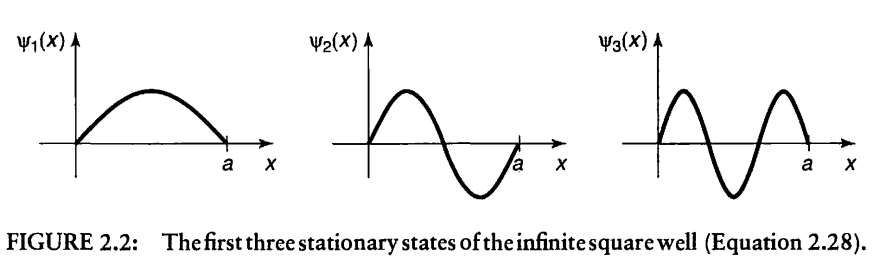
\includegraphics[width=0.8\linewidth]{pics/qm_infinite_square_well.PNG}
    \caption{Wave functions}
\end{figure}
\paragraph{Conductions} (\textbf{pp.1160 ch41 of \cite{book}})
\begin{align}
    P(E) &= \frac{1}{e^{(E-E_F)/kT} +1} 
\end{align}


\section{Atomic Physics}
\label{sec:Atomic-Physics}
\begin{figure}[H]
    \centering
    \includegraphics[width=0.8\linewidth]{pics/{electron-state}.PNG}
    \caption{Electron State (from pp.162 of \cite{book_atomic})}
\end{figure}

\begin{figure}[H]
    \centering
    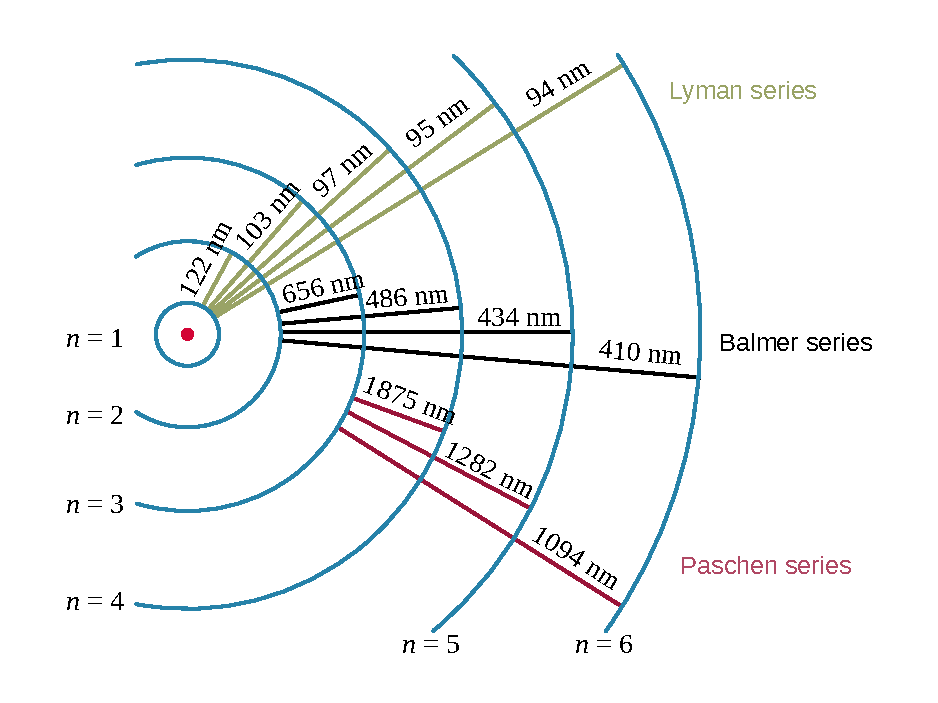
\includegraphics[width=0.8\linewidth]{pics/Hydrogen_spectrum_series.pdf}
    \caption{Hydrogen spectrum series}
\end{figure}
\begin{table}[H]
    \centering
    \caption{Three common decay processes}
    \begin{tabular}{c c}
        Decay name & Process \\
        $\alpha$ & Emitting a Helium Nucleus (two protons and two
        neutrons) \\
        \hline
        $\beta$ & $n\to p+e^- \bar{v_e}$ or $p\to n+e^+ +v_e$ \\
        \hline
        $\gamma$ & Only photon (light ray) emitted \\
        \hline
    \end{tabular}
\end{table}

\section{Standard Model}
Read page 1244 of \cite{book}.
\begin{figure}[ht]
    \centering
    \includegraphics[width=0.8\linewidth]{pics/{Standard-Model-of-Elementary-Particles}.pdf}
    \caption{Standard Model of Elementary Particles (from Wikipedia)}
\end{figure}

\begin{figure}[H]
    \centering
    \includegraphics[width=0.8\linewidth]{pics/{Elementary_particle_interactions_in_the_Standard_Model}.png}
    \caption{Elementary particle interactions in the Standard Model
    (from Wikipedia)}
\end{figure}

\begin{figure}[H]
    \centering
    \includegraphics[width=0.8\linewidth]{pics/{Comprehensive-standard-model-particle-chart}.jpg}
    \caption{Comprehensive standard model particle Chart }
\end{figure}
(from \href{http://electron6.phys.utk.edu/phys250/modules/module%206/images/particle_chart.jpg}{Link})

\begin{figure}[H]
    \centering
    \includegraphics[width=1.0\linewidth]{pics/{Elementary-Particles-concept-map}.pdf}
    \caption{Elementary Particles concept Map}
\end{figure}
\section{Positronium}
\label{sec:Positronium}

\href{https://en.wikipedia.org/wiki/Positronium}{Wiki Positronium}.

Energy:
\begin{equation}
    E_n = -\frac{6.8 \text{eV}}{n^2}
\end{equation}
\section{Common Mathematical Formulae}
\label{sec:Common-Mathematical-Formulae}
\begin{align}
    & \frac{1}{1-x} = 1 + x + x^2 + x^3 + \cdots
\end{align}

\section{Anchor}
\label{sec:anchor}
\begin{thebibliography}{1}
    \bibitem{book} Fundamentals of Physics, Extended Edition. Halliday
    \& Resnick.
    \bibitem{book_atomic} Atomic Physics. Fujia, Yang. (Chinese)
    \bibitem{Griffiths_electrod} Introduction to Electrodynamics, 3rd,
    Griffiths.
    \bibitem{Griffiths_QM} Introduction to Quantum Mechanics, 2nd,
    Griffiths.
    \bibitem{kardar} Kardar. Statistical Physics of Particles. (2007)
\end{thebibliography}
\printnomenclature
\section{License}
The entire content of this work (including the source code
for TeX files and the generated PDF documents) by 
Hongxiang Chen (nicknamed we.taper, or just Taper) is
licensed under a 
\href{http://creativecommons.org/licenses/by-nc-sa/4.0/}{Creative 
Commons Attribution-NonCommercial-ShareAlike 4.0 International 
License}. Permissions beyond the scope of this 
license may be available at \url{mailto:we.taper[at]gmail[dot]com}.
\end{document}
